\xchapter{Síntese de Resultados}{}
\label{discussao}

Este capítulo apresenta 
a síntese dos resultados desta pesquisa através de uma
discussão guiada pelas questões apresentadas na seção \ref{discussao:questoes}.

A seção \ref{sec:discussao} apresenta 
uma discussão geral a respeito da
sustentabilidade técnica do software acadêmico de análise estática,
a partir dos resultados dos estudos apresentados nos Capítulos \ref{estudo1}, \ref{estudo2} e
\ref{estudo3} sobre a publicização, reconhecimento e ciclo de vida do software
acadêmico de análise estática.
A seção \ref{sec:recomendacoes} apresenta recomendações para desenvolvedores e usuários de software acadêmico no sentido de dar corpo a práticas já conhecidas mas que trazem uma grande contribuição a este cenário.
Finalmente, a seção \ref{sec:trabalhosrelacionados} apresenta trabalhos relacionados ao software acadêmico em termos de melhorias no processo de desenvolvimento, reconhecimento e sustentabilidade.

\section{Questões} \label{discussao:questoes}

\newcommand{\QuestaoUm}{
  Como evolui o reconhecimento ao software acadêmico de análise estática
  publicado nas conferências de Engenharia de Software ASE e SCAM?
}
\newcommand{\QuestaoDois}{
  A publicização do software acadêmico de análise estática publicado nas
  conferências de Engenharia de Software ASE e SCAM influencia o seu
  reconhecimento?
}
\newcommand{\QuestaoTres}{
  O ciclo de vida do software acadêmico de análise estática publicado nas
  conferências de Engenharia de Software ASE e SCAM influencia o seu
  reconhecimento?
}
\newcommand{\QuestaoQuatro}{
  Qual o tamanho do software acadêmico de análise estática publicado nas
  conferências de Engenharia de Software ASE e SCAM?
}
\newcommand{\QuestaoCinco}{
  Como evolui o tamanho do software acadêmico de análise estática publicado nas
  conferências de Engenharia de Software ASE e SCAM?
}
\newcommand{\QuestaoSeis}{
  É possível replicar ou reproduzir pesquisas que mencionam software
  acadêmico de análise estática publicado nas conferências de Engenharia de
  Software ASE e SCAM?
}
\newcommand{\QuestaoSete}{
  O software acadêmico de análise estática publicado nas conferências de
  Engenharia de Software ASE e SCAM é sustentável tecnicamente?
}
\newcommand{\QuestaoOito}{
  O software acadêmico de análise estática publicado nas conferências de
  Engenharia de Software ASE e SCAM é útil e maduro suficiente para ser
  utilizado em outras pesquisas?
}

\begin{description}
  \item [Q1] \QuestaoUm
  \item [Q2] \QuestaoDois
  \item [Q3] \QuestaoTres
  \item [Q4] \QuestaoQuatro
  \item [Q5] \QuestaoCinco
  \item [Q6] \QuestaoSeis
\end{description}

\section{Discussão}
\label{sec:discussao}
%A discussão geral é guiada pela questões de pesquisa apresentadas no
%Capítulo \ref{introducao}.

Considerando que esta pesquisa adotou uma estratégia de 
estudo de campo em ambiente natural,
com alto realismo no contexto estudado e,
consequentemente, com baixa generalização,
seus resultados e conclusões são específicos 
ao domínio de análise estática e, em especial,
ao conjunto de projetos observados.

\subsection{Q1 - \QuestaoUm} % taxa crescimento menções

O software acadêmico tem recebido maior atenção na literatura acadêmica com o
passar do tempo; há uma clara evolução no número total de menções a software
acadêmico de análise estática em publicações das bases ACM e IEEE, conforme
Figura \ref{mentions-by-year}.

\begin{figure}[h]
  \centering
  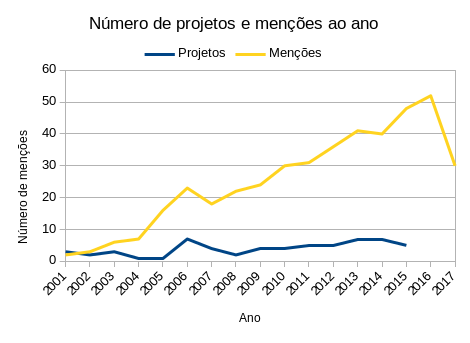
\includegraphics[scale=0.6]{imagens/mentions-projects-by-year.png}
  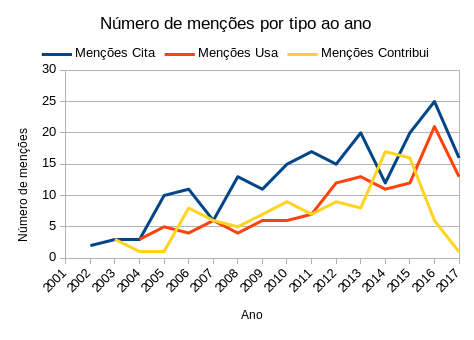
\includegraphics[scale=0.6]{imagens/mentions-type-by-year.png}
  \caption{Número de projetos e menções por tipo ao ano.}
  \label{mentions-by-year}
\end{figure}

Este crescimento, no entanto, pode estar sofrendo influencia do aumento de
projetos, uma vez que há também crescimento no número de projetos a cada ano.
Entretanto, ao isolar os dados, mantendo o número de projetos constante ao longo
do tempo, há um crescimento de 38\% ao ano, conforme Figura
\ref{mentions-trend}.

\begin{figure}[h]
  \center
  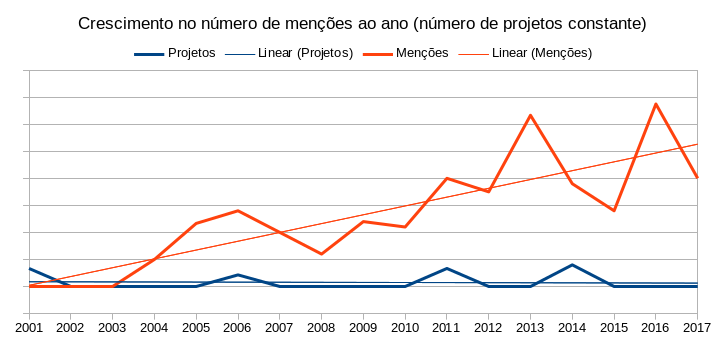
\includegraphics[scale=0.6]{imagens/mentions-trend.png}
  \caption{Crescimento no número de menções ao ano (crescimento médio = 38\%).}
  \label{mentions-trend}
\end{figure}

Entre os 60 projetos de software acadêmico de análise estática estudados, 
13 não possuem reconhecimento acadêmico, ou seja, são
mencionados unicamente no artigo original publicado na ASE ou na SCAM,
que apresentou o software pela primeira vez. 
Os outros 47 projetos possuem maior reconhecimento acadêmico, 
considerando que foram encontradas menções em um ou mais artigos
diferentes da primeira publicação.

%FORA DO ESCOPO: qualidade da citação? 
%FORA DO ESCOPO: como citar software acadêmico?

\subsection{Q2 - \QuestaoDois} % reconhecimento

Há uma evidente relação entre o número de menções e o uso de licenças de
software livre. 
Há 201 menções aos 38 projetos software acadêmico de análise estática sem licença definida, 
enquanto há 228 menções ao 22 projetos com licença, ou seja, 
mesmo com um número menor de projetos, o número de menções encontradas foi 14\% maior, 
conforme Figura \ref{license-vs-mentions}.

\begin{figure}[h]
  \center
  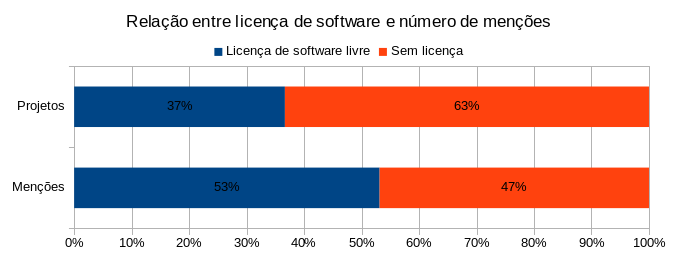
\includegraphics[scale=0.6]{imagens/license-vs-mentions.png}
  \caption{Relação entre o uso de licença de software livre e o número de menções.}
  \label{license-vs-mentions}
\end{figure}

Não foi encontrada relação entre o número de menções e 
outras características do software acadêmico, por exemplo,
disponibilidade para download, linguagem de programação, acesso ao site ou número
de lançamentos.

\subsection{Q3 - \QuestaoTres} % idade média

Os projetos em estágio de {\it Initial development} possuem menos menções em %não deveria haver lançamento, certo?
comparação com o tempo de vida. 
Diferentemente, projetos em estágio de {\it Evolution} ou de {\it Servicing} 
possuem mais lançamentos do que a idade, porém
sendo que o número de menções neste estágio de evolução não é mais disperso. % ou esparso?

A maior parte dos projetos em estágio de {\it Closedown} possui idade superior ao número
de menções, exceto pelos projetos \texttt{s19}, \texttt{s38} e
\texttt{s56} que possuem número de menções bem acima da média geral.
Em especial, o software \texttt{s19} se destaca dentre os projetos com maior número de menções.

Foram encontradas 160 menções para projetos em estágio {\it Closedown},
possivelmente indicando artigos publicados antes do projeto entrar nesta fase ou indicando que o projeto está acessível apenas para os autores destes artigos mas não para o público em geral,
71 menções para projetos em estágio de {\it Evolution} ou {\it Servicing} e 
131 menções para projetos em estágio de {\it Initial development}.

Os projetos \texttt{s19}, \texttt{s38} e \texttt{s56} foram encontrados em um
grande número de menções, incluindo publicações recentes entre os anos de 2016
e 2017, no entanto o fato de serem projetos em estágio {\it Closedown} chama
atenção, uma vez que não estão disponíveis publicamente mas continuam recebendo
atenção da academia, este fato não foi investigado, mas estes projetos são
objetos de estudo interessantes para compreender este fenômeno.

%são os com maior número de
%menções entre os projetos em estágio de
%recentes entre os anos de 2017, 2016 e 2014.
%% QUAIS OS artigos que os citam? Por que?

\subsection{Q4 - \QuestaoQuatro} % tamanho médio

O tamanho médio do software acadêmico de análise estática publicado nas
conferências ASE e SCAM é de 820 módulos. 
Esta média considera a última versão disponível em código fonte de cada projeto.

O tamanho médio dos projetos em estágio de {\it Initial development} é de 595
módulos. Estes projetos são muito menores que os projetos em estágio de {\it Evolution} 
ou  {\it Servicing} que possuem 1261 módulos, em média. 
Os projetos em estágio de {\it Phaseout} ou {\it Closedown} não possuem código disponível e,
portanto, não sabemos seu tamanho.
A Figura \ref{modules-average} apresenta estes números.

\begin{figure}[h]
  \center
  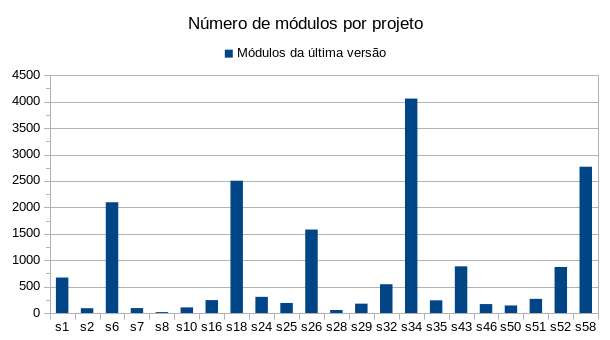
\includegraphics[scale=0.6]{imagens/modules-total.png}
  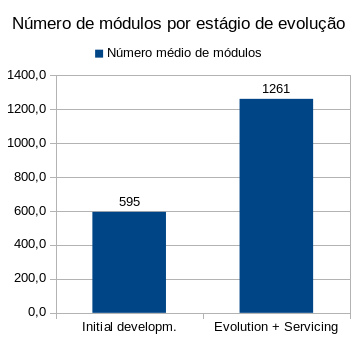
\includegraphics[scale=0.6]{imagens/modules-average.png}
  \caption{Número de módulos por projeto e por estágio de evolução no ciclo de vida.}
  \label{modules-average}
\end{figure}

De 20 projetos em estágio de {\it Initial development}, 
12 projetos tiveram o código fonte analisado. 
Todos os 8 projetos em estágio de {\it Evolution} ou {\it Servicing}
tiveram seu código fonte analisado.
Vale destacar que estes dois estágios foram agregados num único conjunto 
pois possuem características próximas: 
os 2 projetos em estágio de {\it Evolution} estão
muito mais próximos dos projetos em estágio de {\it Servicing} do que 
do projetos em {\it Initial development}. 

\subsection{Q5 - \QuestaoCinco} % evolução no tamanho

Ao analisar a evolução no tamanho (em número de módulos) 
dos projetos em estágio de {\it Servicing}, apresentados na Figura \ref{modules-evolution-servicing},
nota-se um crescimento no número total e médio de módulos
em todos os projetos ao longo dos anos.

\begin{figure}[h]
  \center
  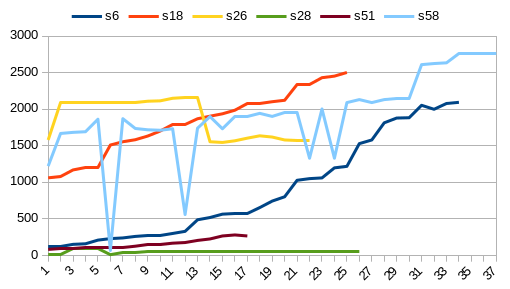
\includegraphics[scale=0.6]{imagens/modules-evolution-servicing.png}
  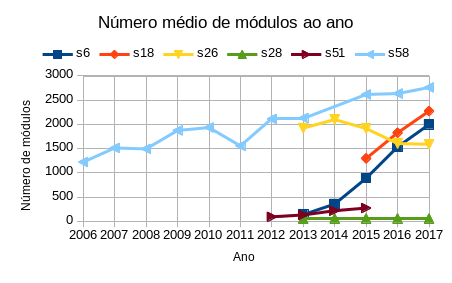
\includegraphics[scale=0.6]{imagens/modules-evolution-average.png}
  \caption{Evolução no número de módulos dos projetos em \textit{Servicing}.}
  \label{modules-evolution-servicing}
\end{figure}

Ao analisar os projetos individualmente, em busca de relação entre
menções e a evolução no tamanho do código fonte (em número de módulos), 
observamos que, para alguns projetos, existe tal relação.
Especulamos que outros projetos podem ter surgido na academia mas 
tiveram seu desenvolvimento posterior externo ao meio científico, 
ao menos para os que foram publicados e indexados nas bases da ACM e do IEEE.

% ACHEI CONFUSO; TENTEI REESCREVER MAS NAO SEI SE FICOU BOM.

\begin{description}

  \item[Software \texttt{s6}.]
    Este projeto teve 5 menções, sendo que em 2015 houve menção do tipo \texttt{Contribui} 
    e em 2017 apenas menções do tipo \texttt{Cita}. 
    Apesar de poucas menções do tipo \texttt{Contribui},
    o projeto apresenta características de estar evoluindo juntamente a atividade
    acadêmica.

  \item[Software \texttt{s18}.]
    Este projeto foi mencionado em apenas 1 artigo em 2012, sendo que o
    primeiro lançamento da versão 2.0 foi em 2015. Este projeto é claramente um
    projeto que ganhou vida própria e seguiu fora da academia.

  \item[Software \texttt{s26}.]
    Este projeto foi mencionado em 7 publicações distintas; em 2014 houve
    menção Contribui, nos anos seguintes possui menções de uso e contribuição.
    A princípio é um projeto com ligação estreita com a atividade acadêmica.

  \item[Software \texttt{s28}.]
    Este projeto está entre os que mais receberam menções, entre 2003 até 2013.
    O projeto tem muitas menções, incluindo contribuições; após 2013, possui apenas
    citações e uso sem novas contribuições. Observa-se uma clara ligação
    entre a evolução do projeto e a atividade acadêmica.

  \item[Software \texttt{s51}.]
    Este projeto teve 4 menções, sendo apenas 1 menção Contribui em 2015,
    e menção Cita e Usa em 2017. O histórico de lançamentos inicia em 2012
    sendo que as primeiras menções aparecem em 2002, o que nos leva a
    questionar: onde estão os lançamentos anteriores a 2012?

  \item[Software \texttt{s58}.]
    Este projeto foi mencionado 11 vezes, sendo apenas 1 menção Contribui em 2010.
    As demais menções são, em grande parte, de uso do software. 
    Entre todos os projetos estudados, este é o que possui maior janela de tempo entre lançamentos, 
    com um histórico de lançamentos de 11 anos. A média dos demais  projetos neste estágio de evolução
    é de apenas 4 anos.

\end{description}

Em resumo, há um crescimento constante no tamanho em número de módulos dos
projetos de software acadêmico de análise estática.
Entretanto, alguns projeto apresentam características de evolução 
totalmente independentes da atividade acadêmica, 
indicando que os seus desenvolvedores, 
apesar de continuar evoluindo os projetos de software,
não tem publicado artigos científicos que os mencionam.

\subsection{Q6 - \QuestaoSeis}

Projetos de software acadêmico de análise estática em estágio de {\it Closedown} 
foram encontrados em menções do tipo Usa em 38 artigos 
e em menções do tipo Contribui em 42 artigos.
Estes projetos não estão disponíveis para download, seja binário ou código fonte, 
e a URL indicada pelos autores não permanece acessível, 
indicando que os resultados de tais artigos não podem ser reproduzidos.
%uma vez que acesso aos artefatos do estudo é requisito necessário para esta tarefa.

Em resumo, as pesquisas reportadas em 80 artigos com menção de Uso ou Contribuição em 
software acadêmico de análise estática publicados nas conferências ASE e SCAM 
não podem ser replicadas ou reproduzidas.

%\subsection{Q7 - \QuestaoSete} % é sustentável?

%FALAR DE ALGUMA RECOMENDACAO / LICAO? AQUI? NA CONCLUSAO?

%ALGUM COMENTARIO SOBRE DCD AQUI? NA CONCLUSAO?

%%---------------------------------------------%%
\section{Recomendações}
\label{sec:recomendacoes}

Os problemas identificados neste estudo podem ser atribuídos, em grande parte,
a baixos orçamentos, limitação de tempo e alta rotatividade entre os
grupos de pesquisa, outros são, possivelmente, ocasionados por questões
culturais \cite{niemeyer2017open}, como, por exemplo, a tímida adoção de
práticas da Ciência Aberta entre pesquisadores.

Ciência Aberta é um movimento que tem por objetivo tornar a pesquisa
científica, seus dados e sua disseminação acessíveis à todos os interessados,
sejam amadores ou profissionais \cite{WikipediaOpenScience}. Sua principal
motivação está em possibilitar a reprodução dos resultados de pesquisas e em
garantir transparência das metodologias utilizadas, isto aumenta o impacto
social das pesquisas e gera economia de tempo e dinheiro para os pesquisadores
e para as instituições \cite{nesta2010open}.

Assim, surge um conjunto de ações que podem ser tomadas pelos diferentes atores
em direção à garantir sustentabilidade nos projetos de software, ações para
praticantes de software, pesquisadores, associações profissionais, educadores,
clientes e usuários. No que tange aos resultados deste estudo, as recomendações
são bastante simples mas muito efetivas.

%para reverter o quadro onde o software acadêmico, sendo considerado
%contribuição científica, deixam de estar disponíveis e inacessíveis aos pesquisadores
%interessados em estudar, aplicar ou contribuir com tais artefatos, algumas recomendações simples
%podem fazer uma grande diferença neste cenário, a maioria delas são práticas amplamente
%recomendadas por iniciativas de Ciência Aberta

Recomendações aos desenvolvedores de software acadêmico \cite{jimenez_four_2017}:

\begin{description}
  \item [Torne o código fonte do software público o mais cedo possível.]

    Desenvolva o código fonte de maneira pública e acessível, utilizar
    repositórios de controle de versão (exemplos, GitHub, Gitlab ou Savannah)
    desde o início do projeto. Quanto mais tempo o projeto seguir um modelo
    fechado, mais difícil se torna abrir. Evitar publicar o software em
    infraestrutura particular ou própria, como por exemplo, servidores da
    universidade, tendem a mudar de endereço ou serem descontinuados.

  \item [Faça o software fácil de ser encontrado e forneça metadados.]

    Forneça metadados a respeito do software através de registros comumente
    adotados pela sua comunidade. Facilitar a descoberta do projeto de software
    e seu código fonte registraodo os metadados a respeito do software em
    locais de registro populares e conhecidos pela comunidade. Metadados devem
    incluir informações de localização do código fonte, contribuidores,
    licença, versão, identificados, referências e como citar o software.

    Boas opções são jornais específicos para software e ferramentas, exemplos:
    JOSS, JORS e SoftwareX. Fornecer instrução sobre como citar o software
    adequadamente, se possível incluir no repositório do projeto um arquvo
    BibTeX \texttt{paper.bib} com os metadados de como deve ser citado.

  \item [Adote uma licença e respeite as licenças de outros pacotes de software.]

    Adote uma licença de software livre adequada para deixar claro como usar,
    modificar e redistribuir o código fonte em termos e condições claros e bem
    definidos. Define a licença de maneira pública e acessível no repositório
    de código fonte, e garanta que o software está em conformidade com as
    licenças de todas as dependências do software.

    Sugestão, preferir especialmente licenças com mecanismo de copyleft, como
    por exemplo: GPL.

  \item [Defina processos claros e transparentes de contribuição, governança e \\ comunicação.]

    Abrir o código do software não significa que o software será desenvolvido
    de maneira pública e colaborativa. Apesar de ser algo desejável,
    recomendações por licenças e práticas comuns de software livre não
    determinam a estratégia para colaborar com a comunidade de desenvolvimento.
    Entretanto, projetos devem ser claros sobre como contribuições devem ser
    feitas e incorporadas tendo modelos de governança transparentes e canais de
    comunicação claros.

  %\item Quando possível, dar preferência a colaborar com projetos existentes em detrimento de iniciar e desenvolver novos projetos.
\end{description}

%Recomendações aos usuários de software acadêmico:
%
%\begin{itemize}
%  \item Sempre indicar a versão do software utilizado na pesquisa.
%  \item Quando possível fazer uso de citação formal ao mencionar software acadêmico, verique se o software fornece sugestão de como ser citado.
%%  \item ao implementar provas de conceitos de novos algoritmos em estudos avaliando e comparando ferramentas enviar quando possível contribuição aos projetos utilizados
%%* evitar manter guardado qualquer código implementado, mesmo que pareça inicialmente não útil para outros
%\end{itemize}

Inevitavelmente alguns projetos de software acadêmico irão continuar sendo
úteis após o primeiro lançamento, alguns terão algumas gerações de melhorias,
outros serão usados na sua versão original sem atualização ou manutenção, e
alguns outros serão lançados e nunca utilizados. Isto é perfeitamente natural,
a comunidade ao redor do software irá decidir qual é o melhor caminho a se
tomar num processo evolutivo \cite{weiner2009astronomical}.

No entanto, sendo o software acadêmico uma parte primordial da produção
científica ele deve estar disponível e continuar disponível para futuras
gerações, dessa forma realizar estudos desta natureza refletindo sobre
o papel do software e evidenciando o quanto ele é tratado em termos
de publicização e reconhecimento é primordial.

No entando algumas lições aprendidas na realização deste estudo nos diz que
atividades de revisão de literatura em busca de menções a software representa
um alto grau de dificuldade e trabalho ``braçal'', este tipo de trabalho seria
simplificada enormemente caso fosse dado ao software um maior reconhecimento e
incentivos a citação formal destes artefatos digitais, ou ao menos, que haja
alguma padronização sobre como citar software, onde seja possível automatizar e
recuperar, de forma segura, a relação entre os projetos, entre artigos e o
software, entre pesquisadores e software, assim como é possível hoje para toda
a produção de literatura.

%prática padronizada sobre como citar software, descobrir na literatura quando
%umm software é citado é um trabalho de certa forma desencorajador, ...

%entre os projetos usando licenças de software livre há um maior número de menções (14\% mais menções que os demais projetos
%FALAR DE DCD aqui? ver últimas frases do RESUMO.

%O ecossistema de software, assim como nos sistemas naturais, necessita de
%fornecimento constante de energia para se manter estável e sustentável, notamos
%no entando que o ecossistema de software acadêmico de análise estática carece
%de investimento, especialmente em termos de contribuição de código fonte, onde

%O desenvolvimento de software sustentável tem sido identificado como um desafio chave no
%campo da Ciência e da Engenharia Computacional. Se sustentabilidade não for levada em
%consideração em projetos de software, não importa qual o domı́nio ou qual o propósito do
%software, perde-se a oportunidade de causar mudanças positivas no planeta e na sociedade
%(BECKER et al., 2014).

%, não sabemos no entanto qual a relação de causa e
%efeito em relação a este maior número de menções aos projetos usando licenças
%livres.

%Alguns projetos de software acadêmico evoluem de maneira independente
%de qualquer atividade acadêmica, com atualizações constantes e lançamentos de
%novas versões ao longo do tempo mas sem nenhuma menção recente na literatura
%acadêmica a respeito do software, 78\% dos projetos estão em estágio inicial de
%desenvolvimento ({\it Initial development}), encerrados ({\it Closedown}) ou
%sendo encerrados ({\it Phaseout}), apenas 13\% dos projetos estão em evolução
%({\it Evolution}) ou provendo serviços ({\it Servicing}).
%
%O tamanho médio do software acadêmico de análise estática em termos de número
%de módulos em estágio {\it Evolution} e {\it Servicing} é duas vezes maior que
%os projetos em {\it Initial development}, a evolução dos projetos mostra um crescimento
%constante no número de módulos no código fonte, confirmando a lei de Lehman de ``Crescimento Contínuo'' do software
%\cite{lehman1997metrics}.

%constantes. Sendo considerados como bons candidados a projetos úteis para uso
%em outras pesquisas.

%%%%%%%%%%%%%%%%%%%%%%%%%%%%%%%%%%%%%%%%%%%%%%%%%%%%

%Observamos que 78\% dos projetos de software acadêmico de análise estática
%encontram-se em estágio inicial de desenvolvimento ({\it Initial development})
%sendo encerrados ({\it Phaseout}) ou já encerrados ({\it Closedown}). Indicando
%que temos neste domínio muitos projetos sem atividade de evolução após a sua
%criação e publicação.

%, este
%crescimento reflete o papel cada vez maior que o software possui na Ciência,
%mas apesar disso há ainda uma porção de software sem qualquer reconhecimento na
%literatura acadêmica, 21\% dos projetos não possuem qualquer menção além do
%artigo inicial onde foram publicados originalmente, 43\% dos projetos são
%utilizados em artigos além da publicação inicial e apenas 28\% recebem
%contribuição em código fonte.

%Este uso é mencionado na literatura academica por meio de citação formal ou in-
%formal (SMITH; KATZ; NIEMEYER, 2016) e está estreitamente relacionado ao sistema
%econômico de reputação cientı́fica, uma vez que menções causam impacto cientı́fico direto
%tanto na publicação quanto no ecossistema de software acadêmico (KATZ, 2014).
%Este impacto direto geralmente justifica o investimentos de novos recursos no ecos-
%sistema, seja para fins de planejamento, por exemplo, uma retrospectiva para avaliar
%investimentos já realizados ou para fins de promoção e evolução do software acadêmico
%(HOWISON et al., 2015).

\section{Trabalhos relacionados}
\label{sec:trabalhosrelacionados}

\citeonline{segal2008developing}
investigam como o desenvolvimento de software acadêmico pode ser melhorado e
enfatiza as diferenças do software acadêmico em relação aos demais tipos de
software, onde o conhecimento sobre o domínio pode muitas vezes incluir temas
avançados e pouco comuns fora do meio científico.

\citeonline{knutson2010report}
ao resumir as conclusões do evento RESER (Workshop on Replication in Empirical
Software Engineering Research) de 2011 cita que ferramentas de software
acadêmico estão indisponíveis ou não são usáveis em estágios não útil, tornando
replicação precisa impraticável.

\citeonline{robles2010replicating} num revisão de 171 artigos do MSR entre 2004 e 2009
em busca de conjunto de dados, artefatos e ferramentas utilizadas nos estudos
necessárias para replicação mostrou que a maioria dos artigos não conseguiram encontrar
as ferramentas mesmo quando o autor explicitamente afirma que fizeram uma.

\citeonline{portillo2012tools}
através de um mapeamento sistemático mostra que grande parte das ferramentas de
software criadas na academia estão em estado inicial de desenvolvimento que
apenas uma pequena porcentagem são testados fora do contexto onde foi
desenvolvido. 

\citeonline{chaturvedi2013tools}
faz uma revisão de literatura entre artigos submetidos ao MSR de 2007 até 2013,
identifica conjunto de dados, ferramentas e técnicas utilizadas pelos autores,
mais da metade dos artigos usam ou criam ferramentas, categoriza as ferramentas
em ferramentas novas, ferramentas tradicionais, protótipos e scripts para
mineração de dados.

\citeonline{barnes2013science}
cria o manifesto {\it Science Code Manifesto} e enfatiza que todo código fonte
escrito especificamente para processar dados de publicações devem estar
disponíveis aos revisores e leitores do paper.

\citeonline{marshall2013tools} num mapeamento sistemático sobre artigos criando
ferramentas de apoio a revisão sistemática no domínio de SE conclui que as
ferramentas encontradas estão em estado inicial de desenvolvimento.

\citeonline{hettrick2014uk} mostra que no reino unido entre todas as áreas da
ciência 56\% dos cientistas estão envolvidos no desenvolvimento de software
acadêmico.

\citeonline{wilson2014best} resume as melhores práticas para melhoria da
manutenibilidade e disponibilidade do software acadêmico desenvolvido por
cientistas.

\citeonline{wilson2014software} num resumo sobre as lições aprendidas em 20
anos da iniciativa {\it Software Carpentry} sobre atividades de melhoria das
habilidades dos pesquisadores com computacao.

\citeonline{amann2015software}
investigam através de uma revisão sistemática de literatura uma década de
publicações e encontram que muito poucos estudos são replicáveis visto que
faltam informações incluindo dados e ferramentas, apenas 20\% dos estudos
possuem ferramentas disponíveis.

\citeonline{momcheva2015software}
num survey com 1142 participantes sobre o uso de software em pesquisas da
astronomia mostrou que 90\% dos cientistas escrevem software e 100\% usam
software em suas pesquisas.

\citeonline{beller2016analyzing} avalia e sugere caminhos para melhorar o
desenvolvimento de ferramentas de análise estática com o objetivo de aumentar a
adoção.

\citeonline{smith2016software} resume recomendações sobre como citar software
na literatura acadêmica com objetivo de encorajar uma ampla adoção e uma
política consistente para citação de software entre as múltiplas disciplinas.

\citeonline{smith2016software} afirma que ``citações aos softwares devem
permitir e facilitar acesso ao software, metadados, documentação, dados e
outros materiais necessários tanto para humanos quanto para máquinas''.

\citeonline{howison2016software}
numa revisão de literatura mostrou que publicações usando softwares como
método, mostrou que apenas 59 mencionavam o uso de softwares de alguma forma,
os demais 31 artigos, apesar de usar software acadêmico, não mencionavam nada a
respeito.

\citeonline{wilson2017good} apresenta um conjunto de boas práticas que todo
pesquisador pode adotar, independentemente do seu nível de habilidade em
computação. Essas práticas passam por gerenciamento de dados, programação,
colaboração com colegas, organização de projetos, tracking work, e escrita da
manuscritos.
%, sao desenhados para uma grande variadade de fontes publicadas do
%noso dia a dia e do nosso trabalho como voluntário organizando workshopts desde
%2010.

%Esta análise para simular um número constante de projetos publicados ao ano foi
%realizada selecionando o número de menções ao ano para um conjunto de no máximo
%3 projetos selecionados aleatoriamente, visto que o número de projetos em
%alguns anos não chega a 3, e para alguns projetos o número de menções é muito
%baixa, repetimos esta seleção algumas vezes até obter um número desejável e
%calculamos a média do número de menções em cada ano.

%, utilizamos várias amostras de menções por
%ano capturando grupos distintos de no máximo 3 projetos e as menções a estes projetos,
%a taxa de crescimento média de menções ao longo dos anos é de 38\%, ou seja,
%permanecendo constante o número de projetos ao ano, as menções irão crescer numa taxa
%de 38\% ao ano na média ...

%Uma questão interessante é a de ``integridade''. 
%O que acontece com os resultados anteriores (publicados)
%se houver um erro ou uma mudança substancial da forma de calcular algo?
%Na prática, só deveríamos permitir refactorings no código 
%de um software acadêmico ou adição de novas funcionalidades?
%(Chris)
%
%An so what?

%O ecossistema de software acadêmico de análise estática sofre de disfunctional ...?
